
%%%%%%%%%%%%%%%%%%%%%%%%%%%%%%%%%%%%%%%%%%%%%%%%%%%%%%%%%%%%%%%%%%%%%%%%%%%
%%% MOTIVATING EXAMPLE
\newcommand{\nilfigure}
{\scalebox{0.75}{
\psset{unit=1mm,nodesep=0mm,labelsep=0.5mm}
\begin{pspicture}(0,0)(1,1)
%\psgrid[xunit=1cm,yunit=1cm,gridwidth=.2pt,subgridwidth=.1pt,subgriddiv=5,subgridcolor=gray,gridcolor=blue](0,0)(1,1)
\putnode{start}{origin}{0}{0}{}
\putnode{stop}{origin}{10}{10}{}
\ncline[offsetB=0,nodesepB=0,linewidth=.7]{-}{start}{stop} %here
\end{pspicture}
}}

\begin{columns}
  \begin{column}{0.5\textwidth}
\begin{boxedminipage}{\textwidth}
 {\scalebox{0.75}{\sf
	\renewcommand{\arraystretch}{1}{
	  \begin{uprogram}
	  \UFL\ \hspace*{-.31\TAL} (\DEFINE\ (\plength\  \lista)
	  \UNL{0}  (\SIF~(\NULLQ \ \lista)
	       0
	       \UNL{1}      ($+$\ 1\ (\plength\ (\CDR\  \lista)))))
          \UNL{0}
          \UNL{0}\ \hspace*{-.31\TAL} (\DEFINE\ (\pfun\  \listb)
	  \UNL{0}  ($+$\ 1\ (\CAR\  \listb)))
%         \UNL{2}\;\;\;\;\;
          \UNL{0}
	  \UNL{0} \hspace*{-.49\TAL} (\LET\ \pz\   $\leftarrow$(\CONS\ ($+$\ $4$ $5$)\
          \UNL{0} \;\;\;\;\;\;\;\;\;\;\;\;\;\;\;\;\;\;\;\;\; (\CONS\ ($+$\ $5$ $2$) \NIL)) \IN
	  \UNL{0} (\SIF\ $*$\ 
	  \UNL{1}  $\pi_1$: (\plength\ \pz\ )
	  \UNL{1}   $\pi_2$: (\pfun\ \pz\ )))
	\end{uprogram}
      }}}
\end{boxedminipage}
  \end{column}
  \begin{column}{0.5\textwidth}
%    Add diagram for liveness of $\pz$ at $\pi_1$  and $\pi_2$
    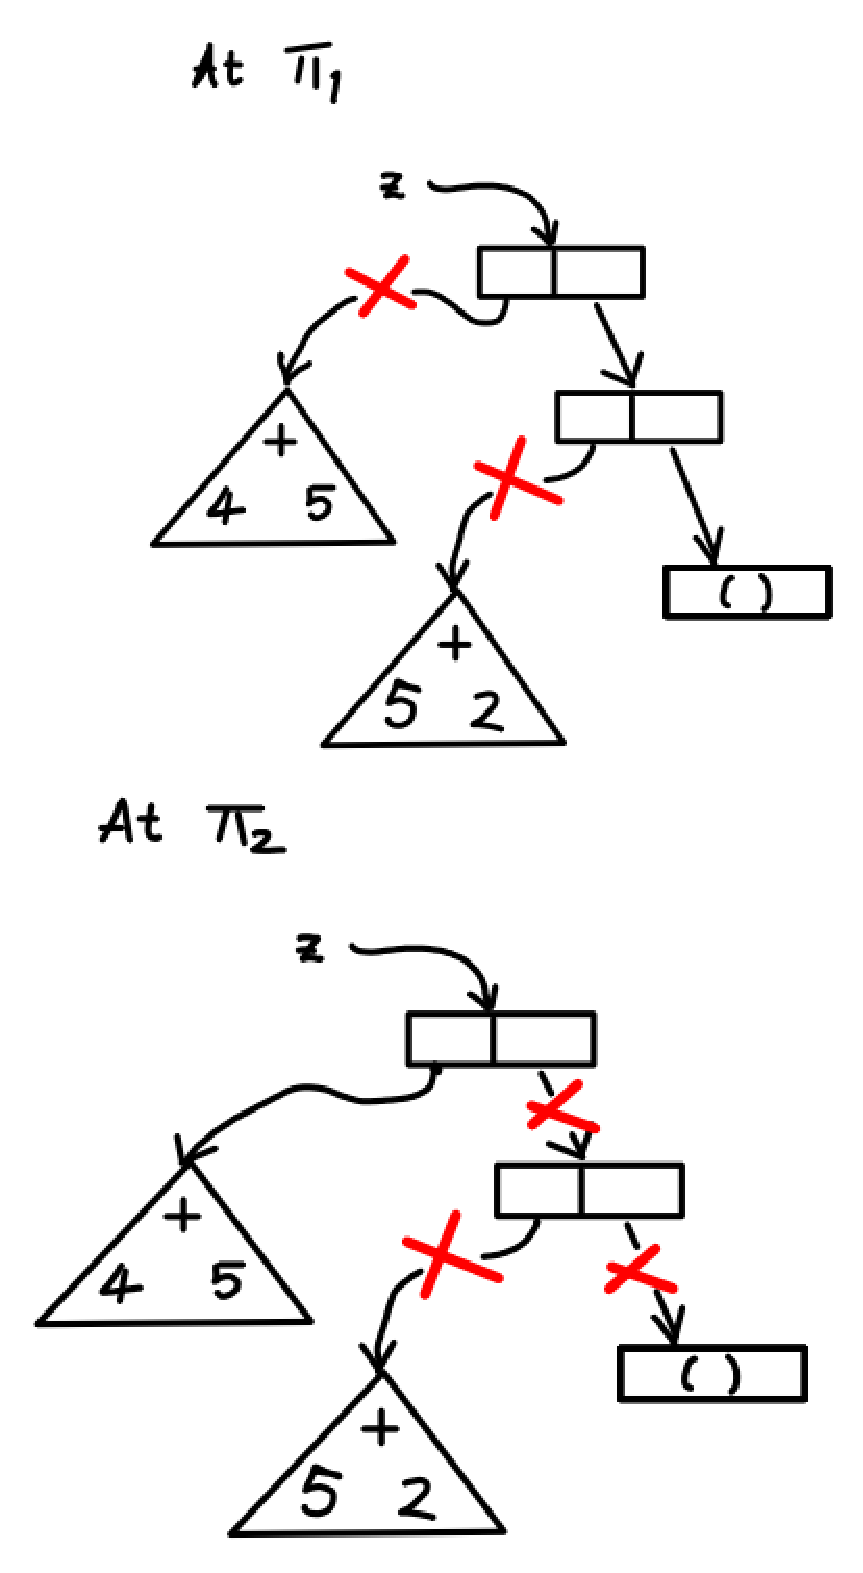
\epsfig{file=mem-graph.eps, height=6.5cm}
    %{mem-graph}
%%       \raisebox{-25mm}{\scalebox{.65}{
%% 	%%%%%%%%%%%%%%%%%%%%%Uday's stuff%%%%%%%%%%%%%%%%%%%%%%%%%
%%       \psset{unit=1mm}
%%       \psset{linewidth=.3mm}
%%       \begin{pspicture}(0,-5)(70,60)
%% %\psgrid[xunit=1cm,yunit=1cm,gridwidth=.2pt,subgridwidth=.1pt,subgriddiv=5,subgridcolor=gray,gridcolor=blue](0,-5)(7,6)
%% 	%\psframe(0,0)(73,60)
%% 	%%%%%%%%%%%%%%%%%%%%%%%%%%%%%%%%%%%%%%%%%%%%%%%%%%%%%%%%%%%%%%%%
%% 	\putnode{o}{origin}{13}{50}{\TwoCells{o1}{o2}}
%% 	\putnode{a}{o}{-10}{-15}{\psframebox{3}}
%% %	\putnode{r}{origin}{26}{38}{}
%% 	\ncline[offsetB=-.5,nodesepB=.1]{*->}{o1}{a}
%%         \putnode{b}{o}{0}{-3}{\psframebox[linestyle=none,framesep=.5]{\scalebox{.63}{\nilfigure}}}
%% %	\ncline[offsetB=-.5,nodesepB=.1]{*->}{o2}{b}
%% 	%\ncline[offsetB=-.5,nodesepB=.1]{->}{o2}{b}
%% 	\putnode{y}{o}{-14}{8}{\psframebox[linestyle=none,framesep=.5]{y}}
%% 	{\nccurve[nodesepB=-.2,angleA=330,angleB=90]{->}{y}{o}}
%% 	\aput[-3.5](.5){\scalebox{1.2}{\psframebox[framesep=.2,linestyle=none,fillstyle=solid,
%% 		  fillcolor=white]{$\times$}}}
%% 	%%%%%%%%%%%%%%%%%%%%%%%%%%%%%%%%%%%%%%%%%%%%%%%%%%%%%%
%% 	\putnode{c}{o}{25}{0}{\TwoCells{c1}{c2}}
%% 	\putnode{d}{c}{10}{-10}{\TwoCells{d1}{d2}}
%% 	\putnode{e}{d}{-13}{-12}{\TwoCells{e1}{e2}}
%% 	\putnode{f}{d}{13}{-12}{\TwoCells{f1}{f2}}
%% %	\nccurve[nodesepB=-.2,angleA=330,angleB=120,linecolor=red]{->}{r}{e}
%% 	\ncline[nodesepB=-.5]{*->}{c2}{d}
%% 	\ncline[nodesepB=-.5,linewidth=.7]{->}{c2}{d}
%% 	\nccurve[ncurv=1,angleA=180,angleB=0]{*->}{c1}{a}
%% 	\aput[-3.5](.2){\scalebox{1.2}{\psframebox[framesep=.2,linestyle=none,fillstyle=solid,
%% 	      fillcolor=white]{$\times$}}}
%% 	\nccurve[nodesepB=-.5,angleA=240,angleB=70]{*->,linecolor=red}{d1}{e}
%% 	\nccurve[nodesepB=-.5,angleA=240,angleB=70,linewidth=.7,linecolor=red]{->}{d1}{e}
%% 	\nccurve[nodesepB=-.5,angleA=300,angleB=110]{*->}{d2}{f}
%% 	\aput[-3.5](.5){\scalebox{1.2}{\psframebox[framesep=.2,linestyle=none,fillstyle=solid,
%% 	      fillcolor=white]{$\times$}}}
%% 	\putnode{w}{c}{-8}{8}{\psframebox[linestyle=none,framesep=.2]{w}}
%% 	\putnode{ww}{c}{15}{8}{\psframebox[linestyle=none,framesep=.2]{z}}
%% 	\nccurve[nodesepB=-.2,angleA=330,angleB=120,linewidth=.7]{->}{w}{c}
%% 	%%%%%%%%%%%%%%%%%%%%%%%%%%%%%%%%%%%%%%%%%%%%%%%%%%%%%%%%%%%%%%%%%%
%% 	\putnode{g}{e}{-8}{-12}{\psframebox{4}}
%% 	\putnode{h}{e}{8}{-14}{\TwoCells{h1}{h2}}
%% 	\putnode{i}{f}{-8}{-11}{\psframebox{6}}
%% %	\putnode{j}{f}{8}{-11}{\psframebox[linestyle=none,framesep=.5]{\NIL}}
%% 	\ncline[offsetB=-.5,nodesepB=.1]{*-}{e1}{e1}
%% 	\ncline[linestyle=dashed,offsetB=-.5,nodesepB=.1,linewidth=.7]{->}{e1}{g}
%%         %here
%%         \putnode{j1}{f}{0}{-3}{\psframebox[linestyle=none,framesep=0]{\scalebox{.63}{\nilfigure}}}
%%         \putnode{j2}{h}{0}{-3}{\psframebox[linestyle=none,framesep=.5]{\scalebox{.63}{\nilfigure}}}

%% %        \aput[-3.2](.6){\scalebox{1.2}{\psframebox[framesep=.1,linestyle=none,fillstyle=solid,
%% %	      fillcolor=white]{$\times$}}} %and here
%% 	\ncline[offsetB=-.5,nodesepB=-.3]{*-}{e2}{e2}
%% 	\ncline[linestyle=dashed,offsetB=-.5,nodesepB=.1,linewidth=.7]{->}{e2}{h} 
%% %	\aput[-3.2](.5){\scalebox{1.2}{\psframebox[framesep=.1,linestyle=none,fillstyle=solid,
%% %	      fillcolor=white]{$\times$}}} %and here

%% 	\ncline[offsetB=-.5,nodesepB=.1]{*->}{f1}{i}
%% 	\ncline[offsetB=-.5,nodesepB=.1]{*->}{f2}{j}
%% 	\nccurve[nodesepB=-.2,angleA=270,angleB=90]{->}{ww}{d}
%% 	\aput[-3.2](.4){\scalebox{1.2}{\psframebox[framesep=.1,linestyle=none,fillstyle=solid,
%% 	      fillcolor=white]{$\times$}}}
%% 	%%%%%%%%%%%%%%%%%%%%%%%%%%%%%%%%%%%%%%%%%%%%%%%%%%%%%%%%%%%%%%%%%%
%% 	\putnode{k}{h}{-8}{-11}{\psframebox{5}}
%% %	\putnode{l}{h}{8}{-11}{\psframebox[linestyle=none,framesep=.5]{\NIL}}
%% 	\ncline[offsetB=-.5,nodesepB=.1]{*-}{h1}{h1}
%% 	\ncline[linestyle=dashed,offsetB=-.5,nodesepB=.1,linewidth=.7]{->}{h1}{k}
%% %	\ncline[offsetB=-.5,nodesepB=.1]{*->}{h2}{l}
%% 	%%%%%%%%%%%%%%%%%%%%%%%%%%%%%%%%%%%%%%%%%%%%%%%%%%%%%%%%%%%%%%%%%%
%%       \end{pspicture}}} 
  \end{column}
\end{columns}

